\chapter{系统测试}

\newcommand{\testcaseheaderrow}{%
\textbf{用例编号} & \textbf{测试功能} & \textbf{操作步骤} & \textbf{预期结果} & \textbf{实际结果} \\}
\newcommand{\testcasecontinuedmark}{%
\multicolumn{5}{r}{续表\arabic{chapter}-\arabic{table}}\\[0.35em]}
\newcommand{\testcaselongtablehead}[2]{%
\caption{#1}
\label{#2}\\
\toprule
\testcaseheaderrow
\midrule
\endfirsthead
\testcasecontinuedmark
\toprule
\testcaseheaderrow
\midrule
\endhead
\bottomrule
\endfoot
\bottomrule
\endlastfoot
}
\newcommand{\resourceusageheaderrow}{%
\textbf{测试场景} & \textbf{持续时间} & \textbf{平均CPU占用} & \textbf{工作集内存} & \textbf{私有内存} & \textbf{结果分析} \\}
\newcommand{\resourceusagecontinuedmark}{%
\multicolumn{6}{r}{续表\arabic{chapter}-\arabic{table}}\\[0.35em]}
\newcommand{\resourceusagelongtablehead}[2]{%
\caption{#1}
\label{#2}\\
\toprule
\resourceusageheaderrow
\midrule
\endfirsthead
\resourceusagecontinuedmark
\toprule
\resourceusageheaderrow
\midrule
\endhead
\bottomrule
\endfoot
\bottomrule
\endlastfoot
}

本章基于当前代码、接口、脚本和打包结果，对 Mini-Chat-Bar 的主要功能进行验证。测试对象包括 Web 端、Electron 桌面端、后端接口、Socket.IO 实时链路以及 AI 问答与总结功能。测试结果一方面用于说明系统已经跑通的主链路，另一方面也用于指出当前版本仍存在的边界和问题。

\section{测试环境与测试方法}

\subsection{测试环境配置}

测试在 Windows 11 64 位单机环境完成。后端通过 \texttt{node server.js} 运行在 \texttt{3000} 端口，Web 端通过 Vite 运行在 \texttt{http://localhost:5173}，数据库采用本地 MongoDB，桌面端测试对象为 \texttt{ccb/dist-electron/win-unpacked/Mini Chat Bar.exe}。为减少历史数据干扰，测试账号、聊天室和消息样本均以 \texttt{ch6} 前缀重新创建，主要环境配置见表~\ref{tab:6-1}。

\begin{table}[!htbp]
\centering
\caption{测试环境配置}
\label{tab:6-1}
\small
\renewcommand{\arraystretch}{1.15}
\setlength{\tabcolsep}{0.8ex}
\begin{tabular}{M{0.14\textwidth}M{0.22\textwidth}p{0.52\textwidth}}
\toprule
\textbf{类别} & \textbf{名称} & \textbf{配置说明} \\
\midrule
硬件 & 处理器 & 12th Gen Intel Core i5-12450H，12 个逻辑处理器 \\
硬件 & 内存 & 16GB 物理内存 \\
硬件 & 存储环境 & 本地 SSD 环境，项目代码、数据库与打包产物均部署在同一测试主机 \\
软件 & 操作系统 & Windows 11 64 位，内核版本 10.0.22631.0 \\
软件 & Node.js & Node.js 24.14.0，npm 11.9.0 \\
软件 & 前端框架 & Vue 3.5.13，Vite 6.3.5，Pinia 3.0.3，Vue Router 4.5.1 \\
软件 & 后端框架 & Express 5.1.0，Socket.IO 4.8.1，Mongoose 8.15.1 \\
软件 & 数据库 & MongoDB 8.0.13，本地数据库名为 \texttt{mini\_chat\_bar} \\
软件 & Redis 环境 & Redis 5.0.14.1，本机已安装，用于辅助验证运行环境完整性 \\
软件 & 桌面端封装 & Electron 36.8.1，打包产物为 \texttt{Mini Chat Bar.exe} \\
软件 & 浏览器 & Chrome 146.0.7680.165 \\
软件 & 辅助工具 & Python 3.13.11、Postman、PowerShell、Chrome DevTools、项目内 \texttt{server/test-chatroom-ai.js} 与 \texttt{server/test-ai-quick.js} 脚本 \\
网络与服务 & 服务端口 & Web 端开发地址为 \texttt{5173} 端口，后端接口与 Socket.IO 服务使用 \texttt{3000} 端口 \\
网络与服务 & 向量检索模式 & \texttt{MessageIndexer} 启动成功，采用本地 hash embedding 模式 \\
\bottomrule
\end{tabular}
\end{table}
\FloatBarrier

\subsection{测试方法与策略}

测试分为两部分进行。一部分是面向用户可见链路的黑盒测试，主要检查登录、聊天、聊天室、收藏、AI 和桌面端提醒是否正常；另一部分使用项目现有脚本和接口记录接口耗时、Socket 广播时延以及资源占用，相关脚本包括 \texttt{server/test-chatroom-ai.js} 和 \texttt{server/test-ai-quick.js}。测试顺序按照“先基础链路、后集成链路、再性能验证”展开，先以 \texttt{/api/user/test} 完成烟雾验证，再依次检查认证、消息、收藏、AI 和并发场景，这种先验证主链路、再记录接口耗时与异常结果的安排也与 RESTful 接口测试研究中的常见做法一致\cite{restfulapitest2025}。

\section{功能测试}

\subsection{功能测试用例设计原则}

功能测试优先覆盖五条最常用链路：登录与会话保持、私聊与聊天室消息、AI 问答与总结、收藏管理以及桌面端提醒。每条用例都给出操作步骤、预期结果和实际结果，保证测试结论能够回溯到具体操作。

\subsection{接口与实时通信测试}

这一部分先验证后端接口和 Socket.IO 事件是否能独立工作。测试时使用 \texttt{ch6userA} 与 \texttt{ch6userB} 两个临时账号完成登录、创建技术聊天室，并通过两条 Socket 连接模拟发送端和接收端；对应测试用例如表~\ref{tab:6-2} 所示。

\renewcommand{\arraystretch}{1.08}
\setlength{\tabcolsep}{0.55ex}
\small
\begin{longtable}{M{0.12\textwidth}p{0.16\textwidth}p{0.18\textwidth}p{0.18\textwidth}p{0.23\textwidth}}
\testcaselongtablehead{接口与实时通信测试用例}{tab:6-2}
IF-01 & 用户登录接口 & 调用登录接口提交用户名和密码 & 返回 200 状态码、JWT 和用户基本信息 & 接口正常返回 JWT，10 次重复调用平均耗时约 58ms \\
IF-02 & 用户信息接口 & 携带 Token 调用 \texttt{/api/user/info} & 返回当前用户标识、昵称、头像和邮箱信息 & 接口 10 次重复调用平均耗时约 5ms，均能返回完整用户对象 \\
IF-03 & 无效 Token 拦截 & 携带无效 Token 调用 \texttt{/api/user/info} & 返回未授权结果，不泄露用户信息 & 接口返回未授权结果，符合权限校验预期 \\
IF-04 & 聊天室消息发送接口 & 调用聊天室消息发送接口提交文本消息 & 返回消息对象，包含消息编号、发送者和时间信息 & 接口 15ms 内返回成功，消息被写入数据库 \\
IF-05 & 聊天室消息列表读取 & 调用消息列表接口读取最近记录 & 返回消息列表，条数正确且时间顺序正确 & 列表接口稳定返回 2 条以上记录，时间线与发送顺序一致 \\
IF-06 & 私聊实时通信事件 & 发送端触发 \texttt{private-message}，接收端监听同名事件 & 接收端能够实时收到完整消息内容 & 接收端在 6ms 内收到测试消息，内容与发送端一致 \\
IF-07 & Socket 重连恢复 & 重连后再次触发 \texttt{private-message} 事件 & 重连后仍可接收实时消息，且不重复投递 & 接收端重连后约 8ms 内恢复收消息能力，未出现重复消息 \\
IF-08 & AI 问答接口 & 调用 AI 问答接口提交技术问题 & 返回结构化 JSON，包含回答正文和历史来源信息 & 单次请求耗时约 19.5s，返回约 1500 字回答；测试语料较少时历史来源列表为 0 \\
\end{longtable}
\normalsize
\FloatBarrier

图~\ref{fig:6-1} 汇总了这一部分的主要测试证据，包括接口返回结果、服务端终端输出、Socket 事件记录和 AI 返回界面，可直接对应表~\ref{tab:6-2} 中的测试项。

\begin{figure}[H]
\centering
\begin{subfigure}[t]{0.48\textwidth}
\centering
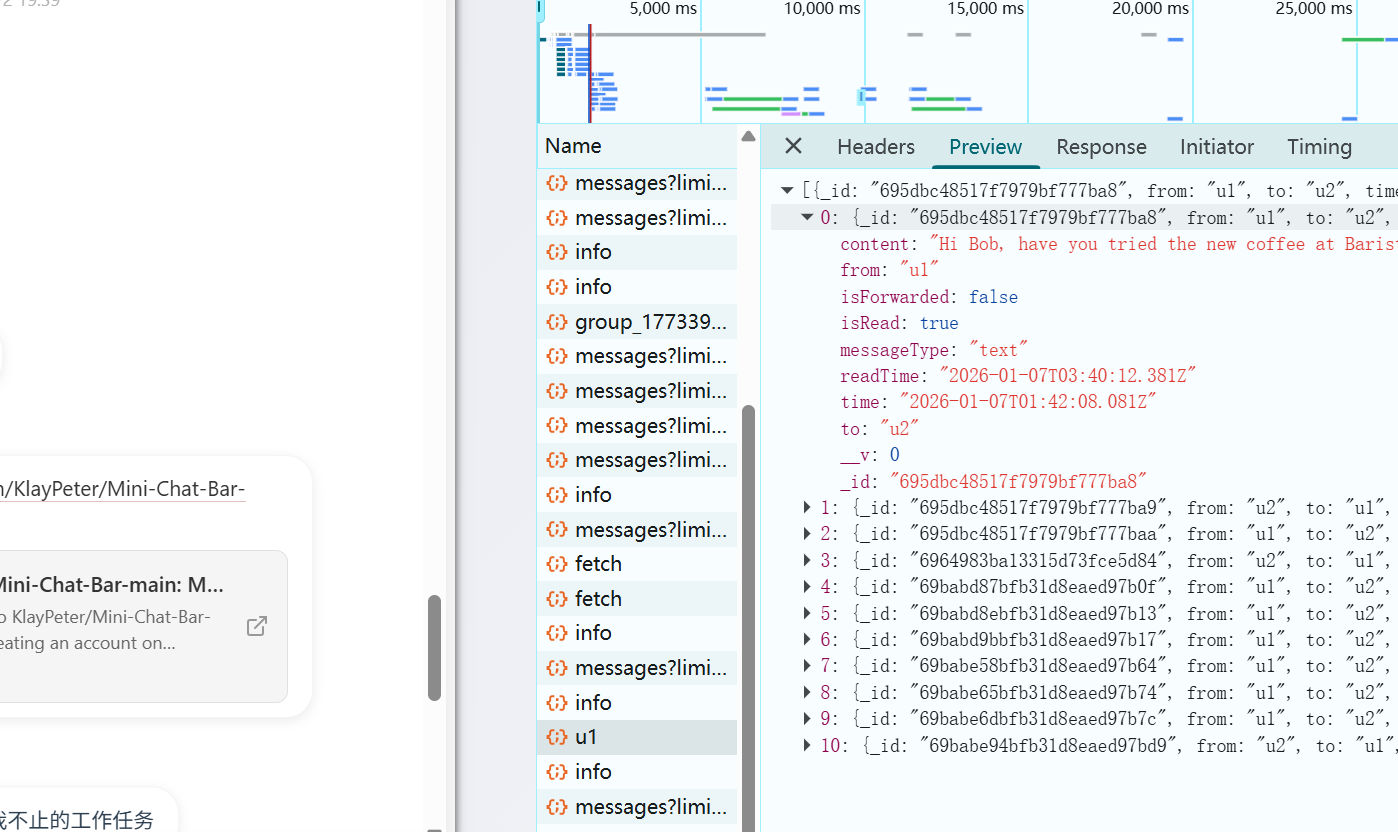
\includegraphics[width=\linewidth,height=4.8cm,keepaspectratio]{img/图6-1_接口返回结果.png}
\caption{接口返回结果}
\end{subfigure}
\hfill
\begin{subfigure}[t]{0.48\textwidth}
\centering
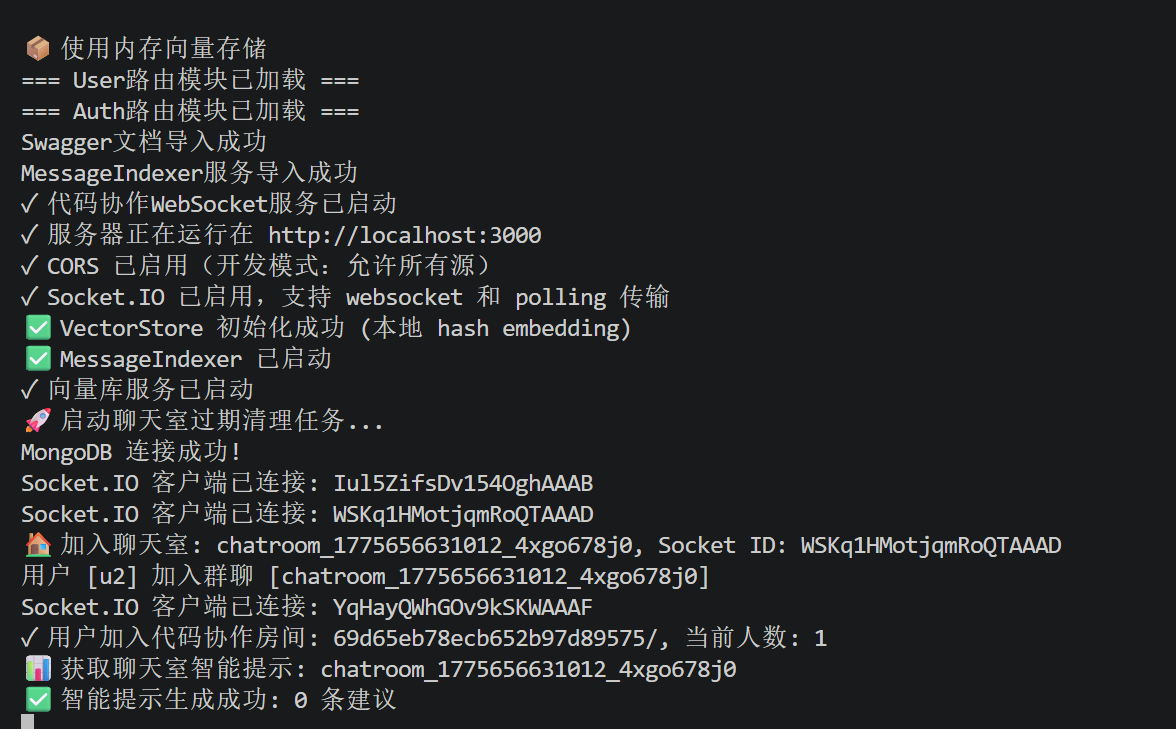
\includegraphics[width=\linewidth,height=4.8cm,keepaspectratio]{img/图6-1_后端终端输出.png}
\caption{后端终端输出}
\end{subfigure}

\vspace{0.6em}

\begin{subfigure}[t]{0.48\textwidth}
\centering
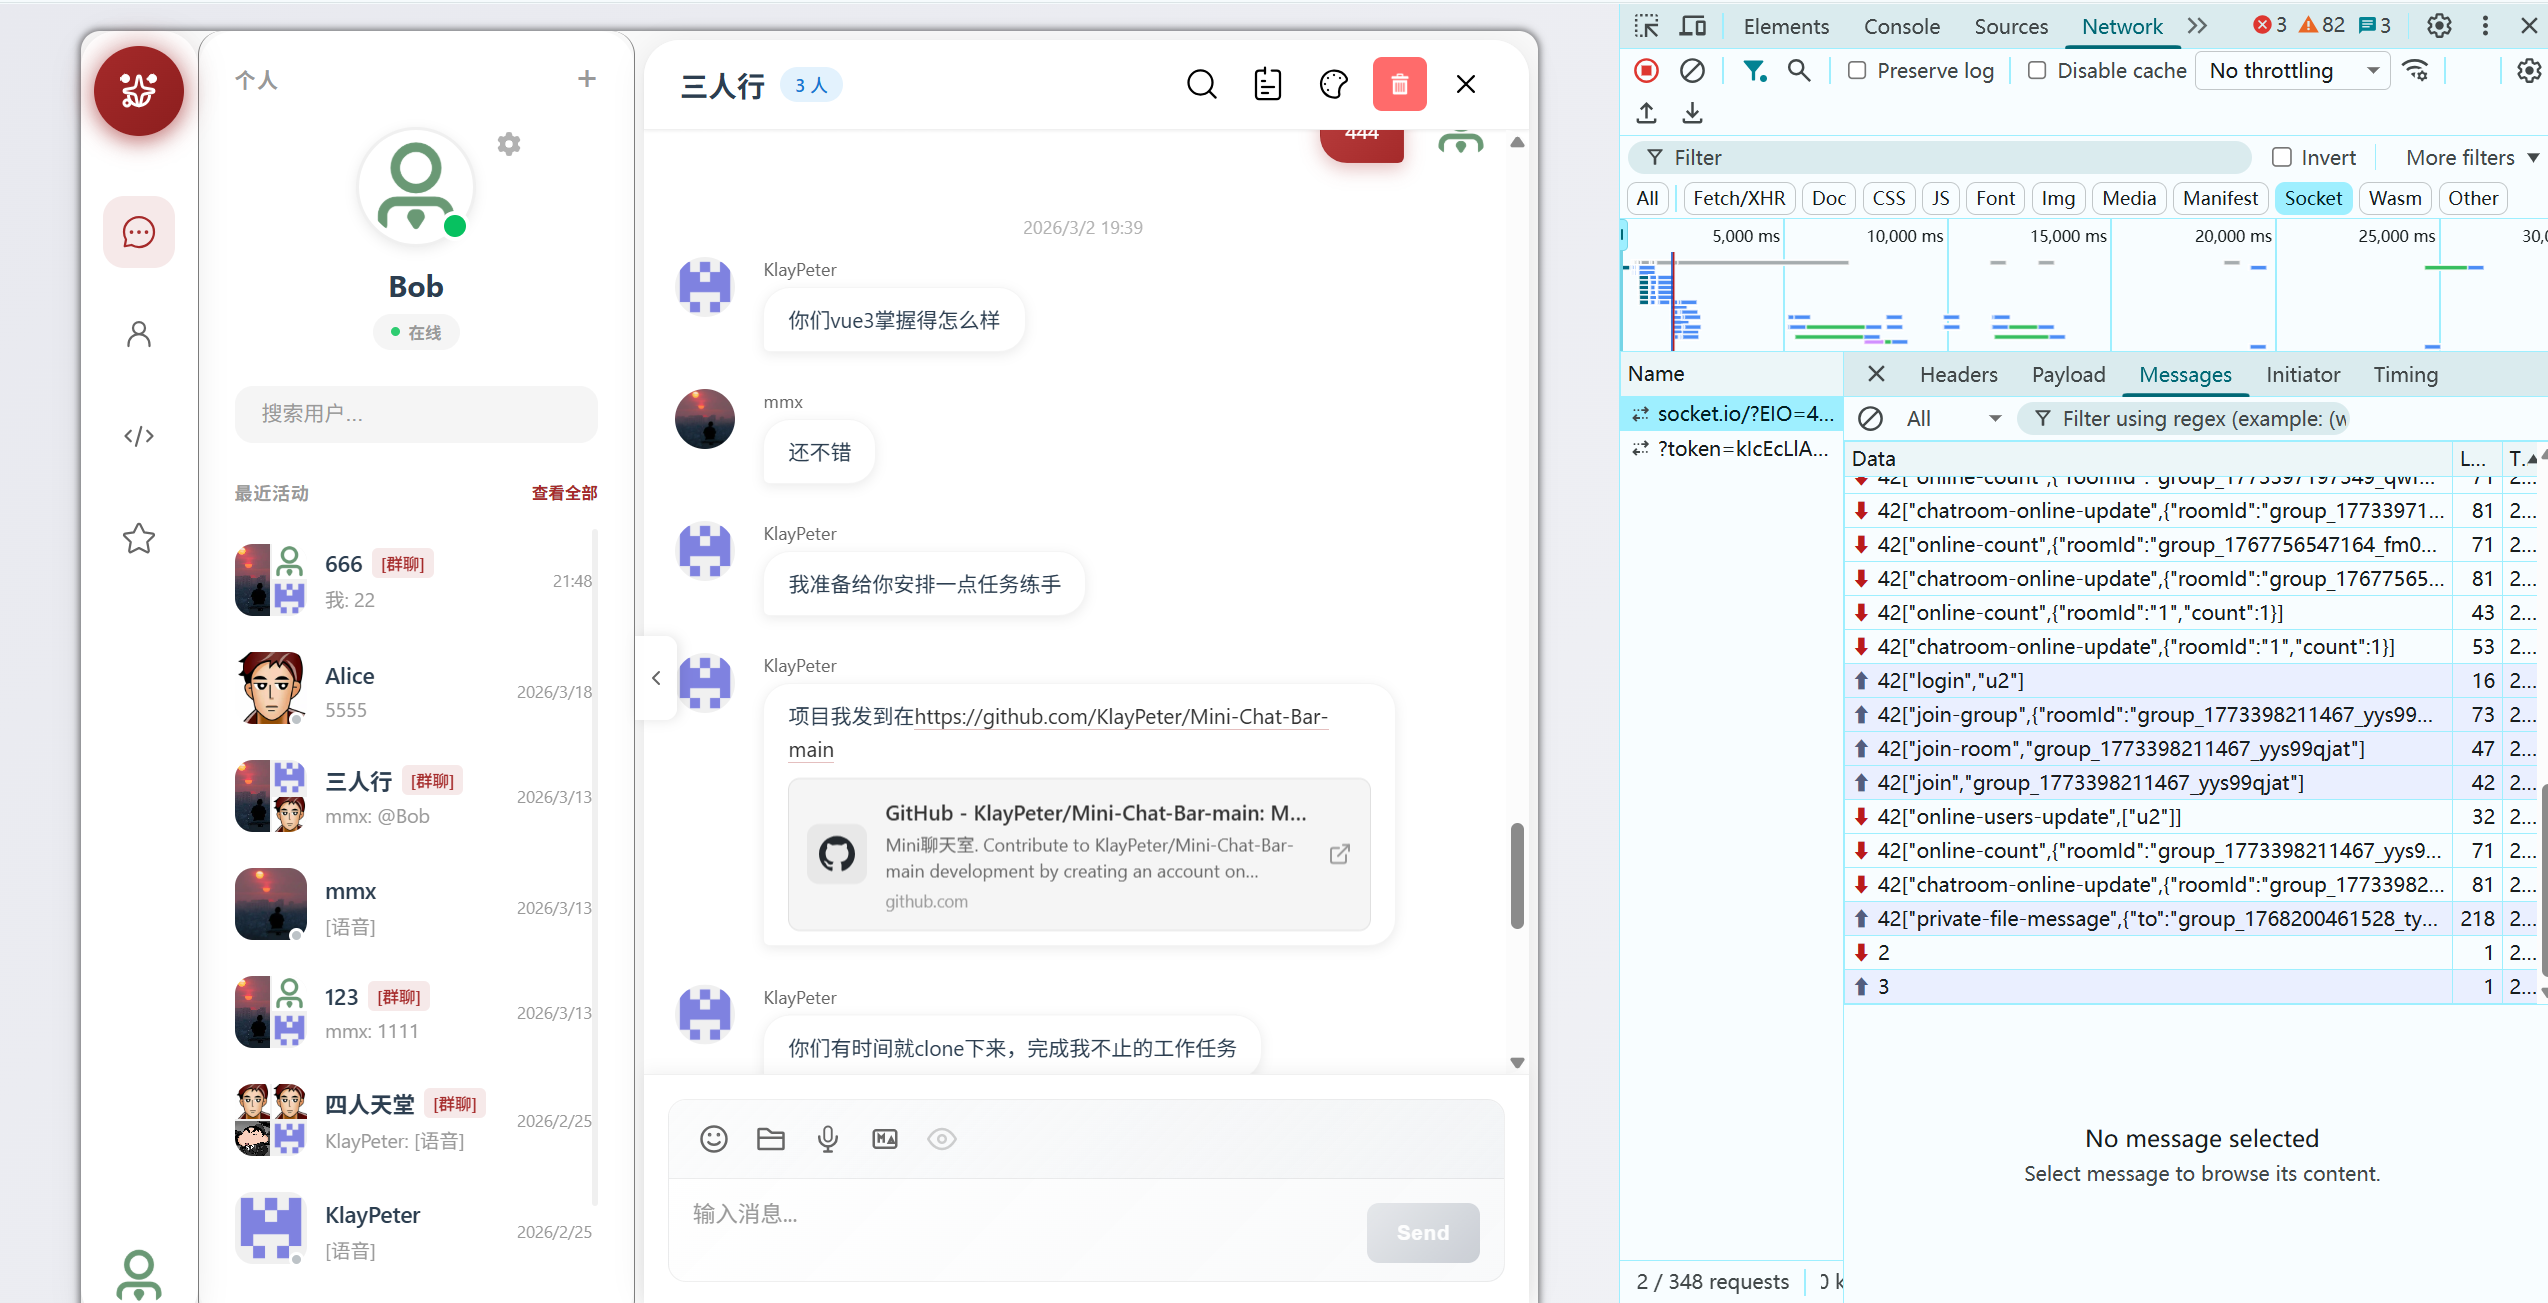
\includegraphics[width=\linewidth,height=4.8cm,keepaspectratio]{img/图6-1_Socket通信记录.png}
\caption{Socket 通信记录}
\end{subfigure}
\hfill
\begin{subfigure}[t]{0.48\textwidth}
\centering
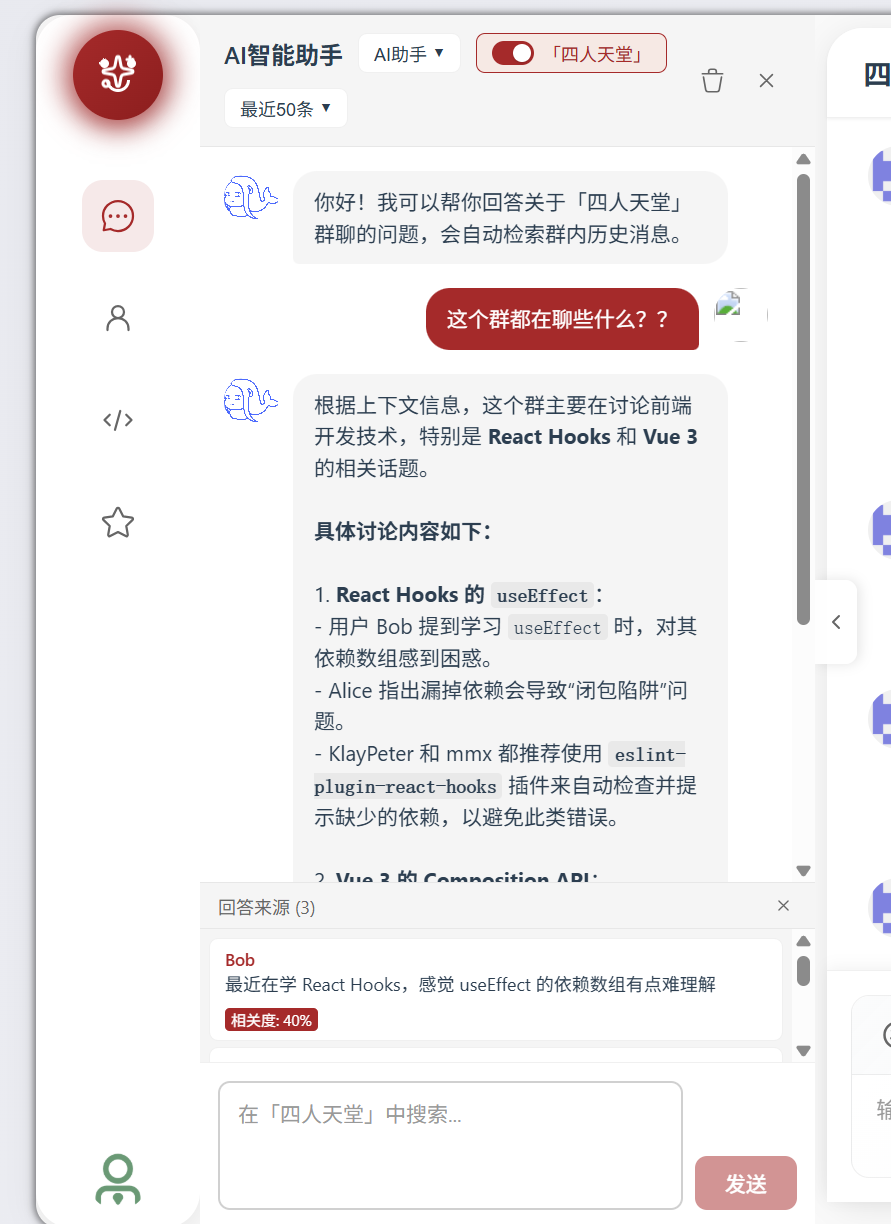
\includegraphics[width=\linewidth,height=4.8cm,keepaspectratio]{img/图6-1_AI返回结果.png}
\caption{AI 返回结果}
\end{subfigure}
\caption{接口与实时通信测试证据组合图}
\label{fig:6-1}
\end{figure}
\FloatBarrier

从表~\ref{tab:6-2} 和图~\ref{fig:6-1} 可以看出，登录、资料读取、聊天室消息写入和私聊事件投递都已跑通。本地环境下 \texttt{private-message} 接收时延约为 6ms；AI 问答接口能够返回完整结果，但耗时明显高于普通业务接口。

\subsection{Web端功能测试}

\subsubsection{登录与会话保持测试}

Web 端先从登录和会话保持开始验证，因为后续所有页面都依赖这条链路。测试覆盖密码登录、验证码登录、会话保持、错误凭证拦截和未登录路由保护。实测显示，登录后可从 \texttt{/login} 跳转至 \texttt{/chats} 并写入本地会话，刷新后仍能保持登录态；清空本地信息后访问受保护路由会重新跳回登录页，见表~\ref{tab:6-3}。

\renewcommand{\arraystretch}{1.08}
\setlength{\tabcolsep}{0.55ex}
\small
\begin{longtable}{M{0.12\textwidth}p{0.16\textwidth}p{0.18\textwidth}p{0.18\textwidth}p{0.23\textwidth}}
\testcaselongtablehead{Web端登录功能测试用例}{tab:6-3}
WEB-01 & 密码登录 & 在登录页输入邮箱和密码并提交 & 页面跳转到主聊天界面，显示当前用户信息 & 登录成功，主界面正常显示，接口耗时与接口测试结果一致 \\
WEB-02 & 验证码登录 & 请求验证码后输入正确验证码并提交 & 登录成功并建立本地会话 & 验证码发送成功，60s 倒计时正常，登录后完成页面跳转 \\
WEB-03 & 会话保持 & 刷新浏览器页面并重新访问主界面 & 路由守卫识别到有效 Token，不跳回登录页 & 刷新后仍停留在主界面，会话保持正常 \\
WEB-04 & 错误凭证拦截 & 输入错误密码后提交表单 & 登录失败并给出错误提示，不进入系统主页 & 页面弹出密码错误提示，未发生错误跳转 \\
WEB-05 & 空表单校验 & 不输入邮箱或密码直接点击登录 & 前端给出必填提示，不发起无效登录流程 & 页面提示“请输入邮箱和密码”，未进入成功登录流程 \\
WEB-06 & 未登录路由拦截 & 直接访问收藏页或聊天室页等受保护路径 & 自动跳转回登录页并清除残留本地数据 & 访问受保护路由时立即跳转至 \texttt{/login}，残留本地数据被清理 \\
\end{longtable}
\normalsize
\FloatBarrier

这一部分重点记录了本地存储、页面跳转和路由守卫状态，相关证据统一汇总到图~\ref{fig:6-2}。测试结果说明登录页、路由守卫和本地会话保持都已正常工作，错误凭证和空表单也会被前端拦截，没有出现异常跳转。

\subsubsection{聊天与聊天室功能测试}

聊天与聊天室测试直接围绕当前前端界面展开，验证对象包括 \texttt{Chat\-View.vue}、\texttt{Con\-tent.vue}、\texttt{ChatRoom\-List\-Panel.vue} 和 \texttt{ChatRoom\-Detail.vue}。这一部分重点检查消息是否写库、历史记录是否能回读、房间是否能正常创建和加入，见表~\ref{tab:6-4}。

\renewcommand{\arraystretch}{1.08}
\setlength{\tabcolsep}{0.55ex}
\small
\begin{longtable}{M{0.12\textwidth}p{0.16\textwidth}p{0.18\textwidth}p{0.18\textwidth}p{0.23\textwidth}}
\testcaselongtablehead{Web端聊天与聊天室功能测试用例}{tab:6-4}
WEB-07 & 私聊消息发送 & 在聊天界面选择联系人并发送文本消息 & 对话区新增消息，后端保存对应私聊记录 & 消息即时回显，数据库中生成对应私聊记录 \\
WEB-08 & 私聊历史回读 & 重新进入会话或刷新页面后加载消息列表 & 能读取历史消息并按时间顺序显示 & 刷新后历史消息正常加载，最新消息位于列表末尾 \\
WEB-09 & 创建公开技术聊天室 & 在聊天室页填写房间名称、技术方向和公开加入方式后提交 & 生成新聊天室并自动出现在房间列表中 & 测试房间创建成功，列表基础回读时可见新建房间 \\
WEB-10 & 加入密码聊天室 & 在聊天室列表中选择目标房间并输入密码加入 & 加入成功并看到历史消息或系统加入提示 & 输入正确密码后成功进入房间，并生成加入系统消息 \\
WEB-11 & 聊天室消息显示与空消息拦截 & 分别发送正常文本和仅空格内容 & 正常消息成功显示，空消息被拦截不提交 & 文本消息正常显示，空白输入不会触发发送，消息顺序一致 \\
\end{longtable}
\normalsize
\FloatBarrier

测试过程中补充记录了私聊回读、公开聊天室创建、密码房间加入和空消息拦截四条关键路径，相关证据统一汇总到图~\ref{fig:6-2}。结果显示，私聊发送、历史回读、公开房间创建和密码房间加入都能正常完成，空白消息也会在前端被拦截，没有进入后端链路。

\subsubsection{AI问答与总结功能测试}

AI 功能测试主要检查三条链路：聊天室内直接提问、输入 \texttt{@AI} 的快捷提问，以及讨论总结生成。为保证结果可重复，测试前先向房间写入 4 条样本消息。实测 AI 问答约 19.5s、总结约 11.8s，刷新后回复仍可回读，见表~\ref{tab:6-5}。

\renewcommand{\arraystretch}{1.08}
\setlength{\tabcolsep}{0.55ex}
\small
\begin{longtable}{M{0.12\textwidth}p{0.16\textwidth}p{0.18\textwidth}p{0.18\textwidth}p{0.23\textwidth}}
\testcaselongtablehead{Web端AI功能测试用例}{tab:6-5}
WEB-12 & AI 问答 & 在聊天室中提交技术问题并等待返回 & 页面显示思考状态，随后插入 AI 回复消息 & AI 接口调用成功，约 19.5s 后返回约 1500 字回复，页面可继续交互 \\
WEB-13 & 讨论总结 & 打开总结对话框并触发总结生成 & 返回结构化总结内容，能够概括主要讨论点 & 总结生成成功，耗时约 11.8s，基于 5 条消息生成约 600 字摘要 \\
WEB-14 & \texttt{@AI} 快捷提问 & 在输入框中插入 \texttt{@AI} 前缀问题并发送 & 自动触发 AI 问答并在消息区追加回复 & 输入 \texttt{@AI} 后先写入用户问题，再生成 AI 回复，流程闭环正常 \\
WEB-15 & 低语料场景问答 & 提交一个与当前技术方向相关的问题 & 仍能返回有效回答，不因历史消息较少而报错 & 样本消息较少时仍返回有效回答，但历史来源列表为 0 \\
WEB-16 & AI 回复持久化 & 刷新聊天室详情页并重新拉取消息 & AI 回复仍可从历史消息中读取并显示 & 刷新后 AI 回复仍可从历史消息中读取，说明结果已成功落库 \\
\end{longtable}
\normalsize
\FloatBarrier

测试中补充记录了从提交问题到结果落库的全过程，相关证据统一汇总到图~\ref{fig:6-2}。从测试结果看，AI 问答、\texttt{@AI} 快捷提问和总结生成都已跑通，且 AI 回复会落库，刷新后仍能回读。当前主要限制仍是耗时受外部模型服务影响，低语料场景下历史来源列表也可能为空。

\subsubsection{收藏功能测试}

收藏测试围绕添加收藏、状态同步、列表回读、取消收藏和组合筛选展开。该模块与消息列表和聊天室状态都有联动，因此除了接口返回，还需要观察前端回显是否正确。基础收藏与回读均正常，但一次带 \texttt{messageType=chatroom} 与关键字的组合查询返回了 500 状态码，见表~\ref{tab:6-6}。

\renewcommand{\arraystretch}{1.08}
\setlength{\tabcolsep}{0.55ex}
\small
\begin{longtable}{M{0.12\textwidth}p{0.16\textwidth}p{0.18\textwidth}p{0.18\textwidth}p{0.23\textwidth}}
\testcaselongtablehead{Web端收藏功能测试用例}{tab:6-6}
WEB-17 & 添加收藏 & 对目标消息执行收藏操作 & 收藏成功，生成消息快照和标签备注信息 & 收藏接口调用成功，消息被写入收藏集合 \\
WEB-18 & 收藏状态同步 & 观察消息右键菜单或收藏状态标记 & 已收藏消息能够被正确识别与回显 & 返回消息区后星标状态正确，重新进入聊天室仍能识别已收藏消息 \\
WEB-19 & 收藏列表回读 & 进入收藏页读取默认列表 & 能看到刚收藏的消息记录及来源信息 & 基础列表查询返回 1 条记录，能够显示测试消息 \\
WEB-20 & 取消收藏 & 在收藏详情页点击“取消收藏”并刷新列表 & 收藏记录被删除，消息恢复未收藏状态 & 取消后收藏页记录消失，聊天室中的收藏状态同步取消 \\
WEB-21 & 收藏组合筛选 & 在收藏页同时使用会话类型和关键字进行筛选 & 正常返回匹配记录 & 一次组合查询返回 500 状态码，说明筛选逻辑仍需进一步校验 \\
\end{longtable}
\normalsize
\FloatBarrier

收藏测试重点记录了“收藏动作触发 - 列表回读 - 状态回显 - 取消收藏 - 组合筛选异常”这一闭环，代表性画面统一汇总到图~\ref{fig:6-2}。其中，聊天室代码协作测试界面对应前端多消息与代码块混排场景，AI 问答结果和讨论总结结果分别对应本节的 WEB-12 至 WEB-16 测试项，设置与主题切换回显则用于补充说明前端交互状态在功能测试过程中的一致性。常规路径已经可用：消息收藏后能在收藏页读到，也能正确取消。问题出现在组合筛选，带 \texttt{messageType=chatroom} 和关键字的查询仍然返回 500，这部分还需要单独排查。

\begin{figure}[H]
\centering
\begin{subfigure}[t]{0.48\textwidth}
\centering
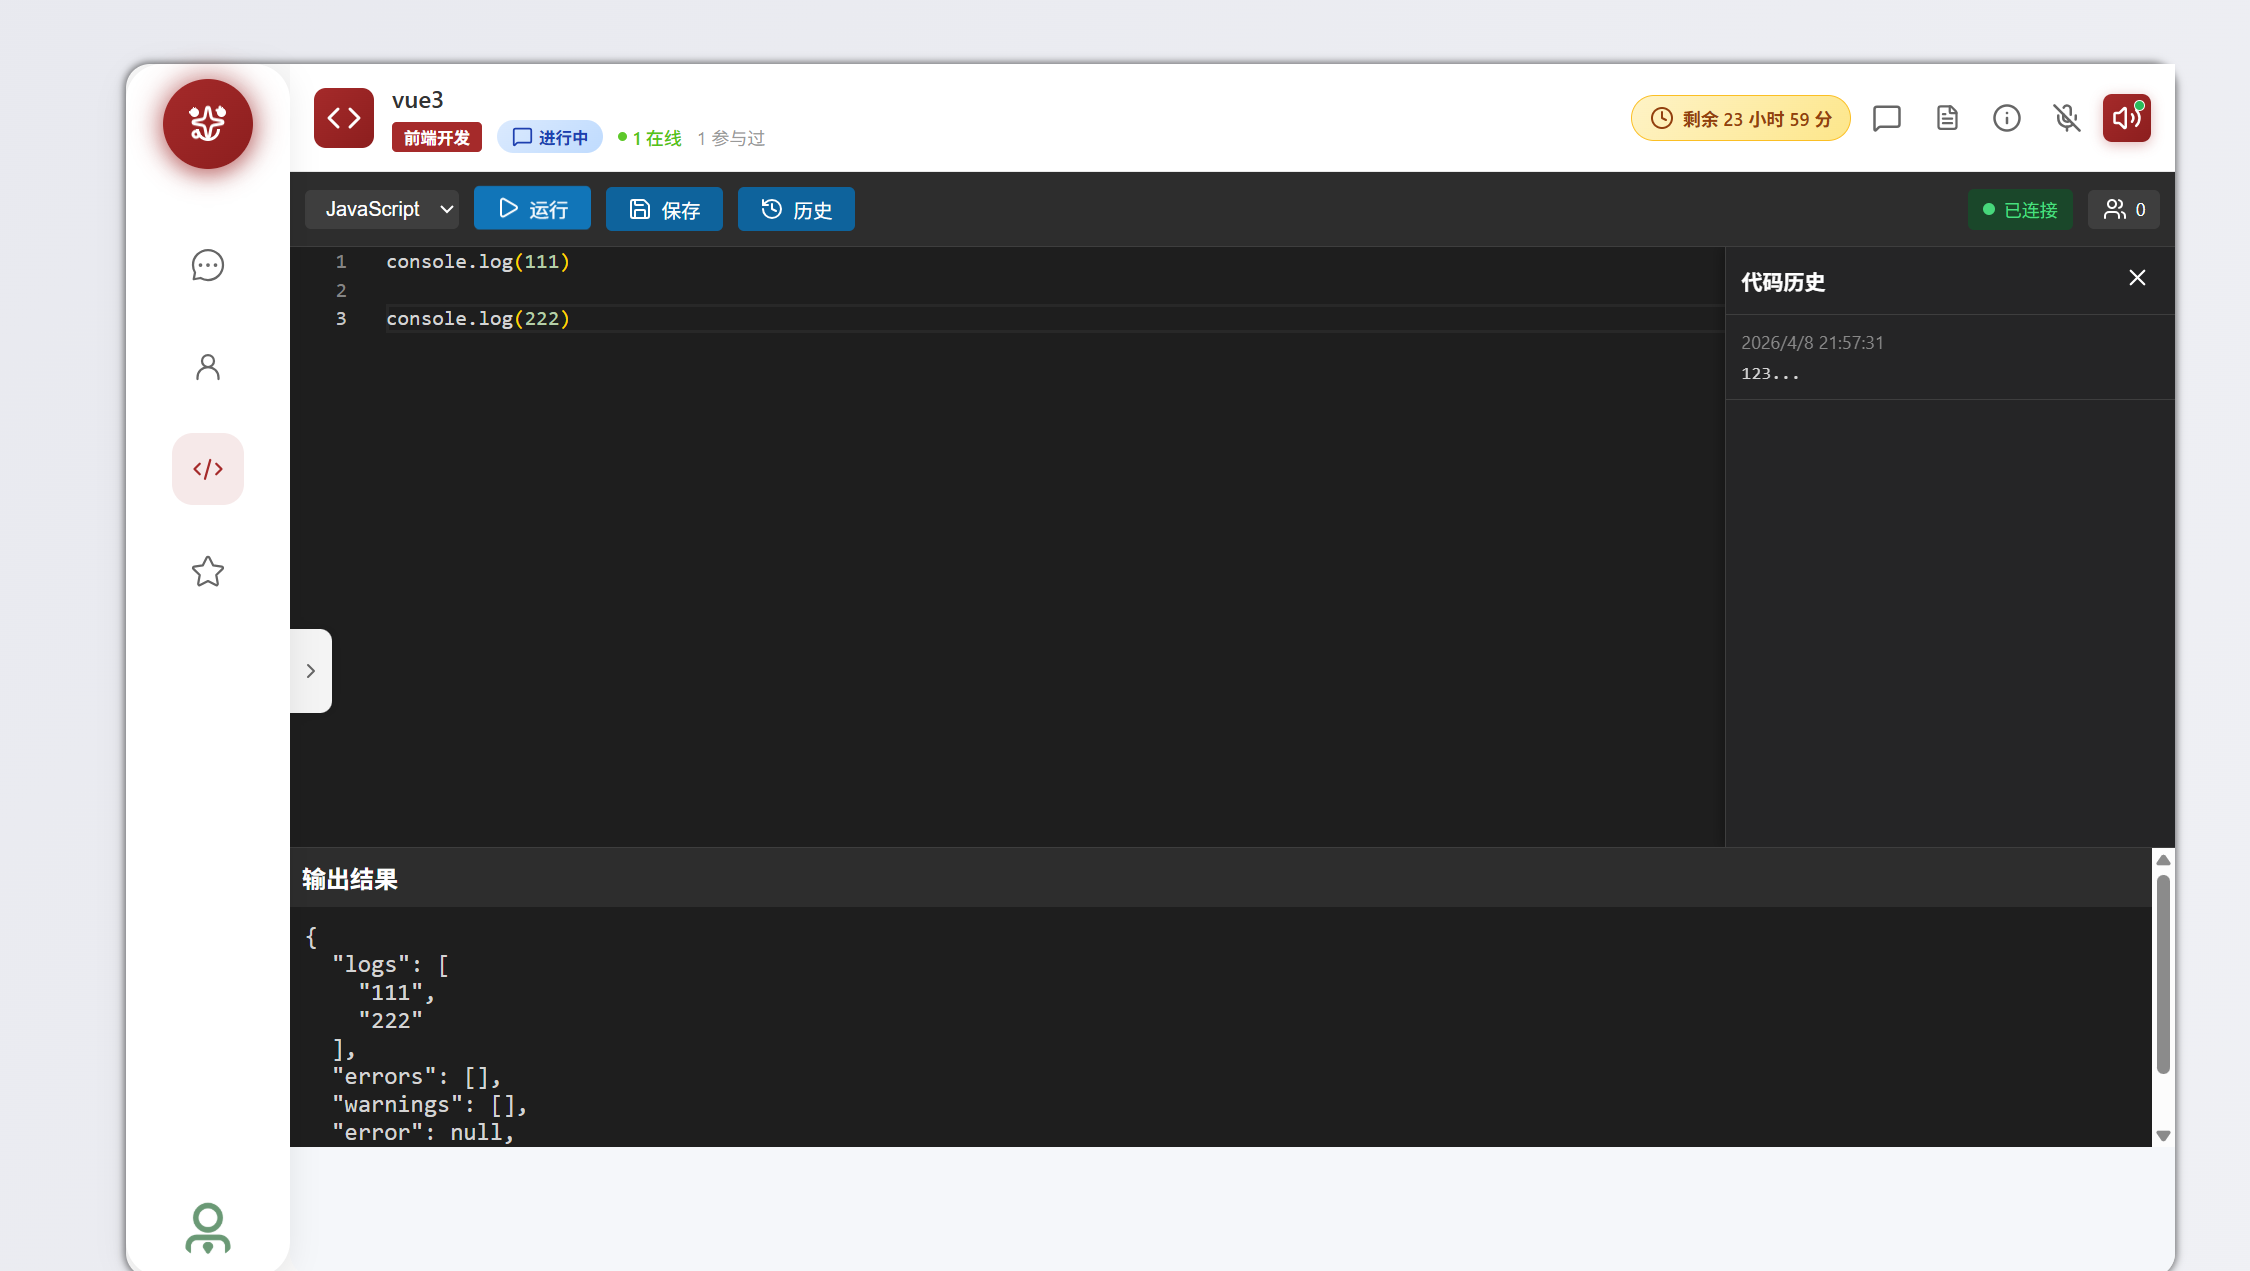
\includegraphics[width=\linewidth,height=4.8cm,keepaspectratio]{img/图6-2_聊天室代码协作测试.png}
\caption{聊天室代码协作测试}
\end{subfigure}
\hfill
\begin{subfigure}[t]{0.48\textwidth}
\centering
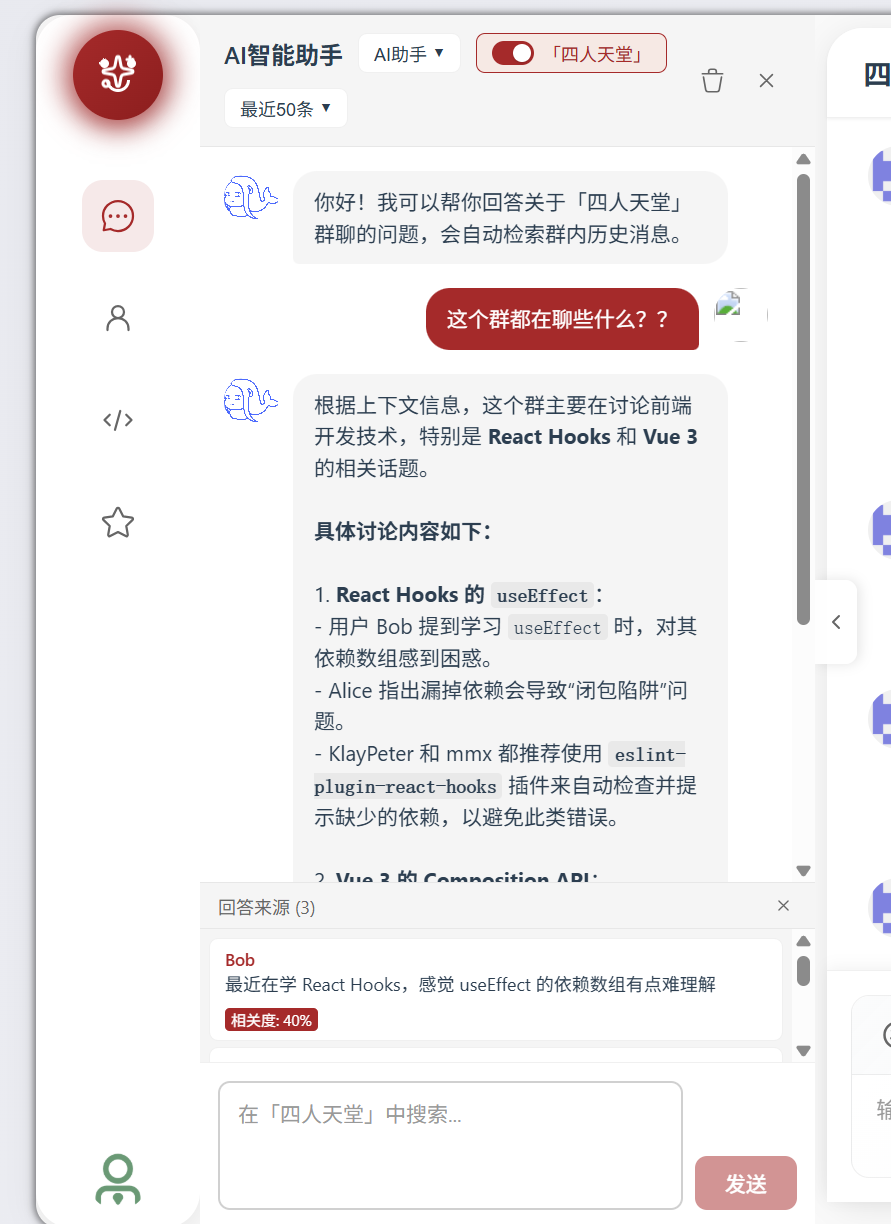
\includegraphics[width=\linewidth,height=4.8cm,keepaspectratio]{img/图6-2_AI问答结果.png}
\caption{AI 问答结果}
\end{subfigure}

\vspace{0.6em}

\begin{subfigure}[t]{0.48\textwidth}
\centering
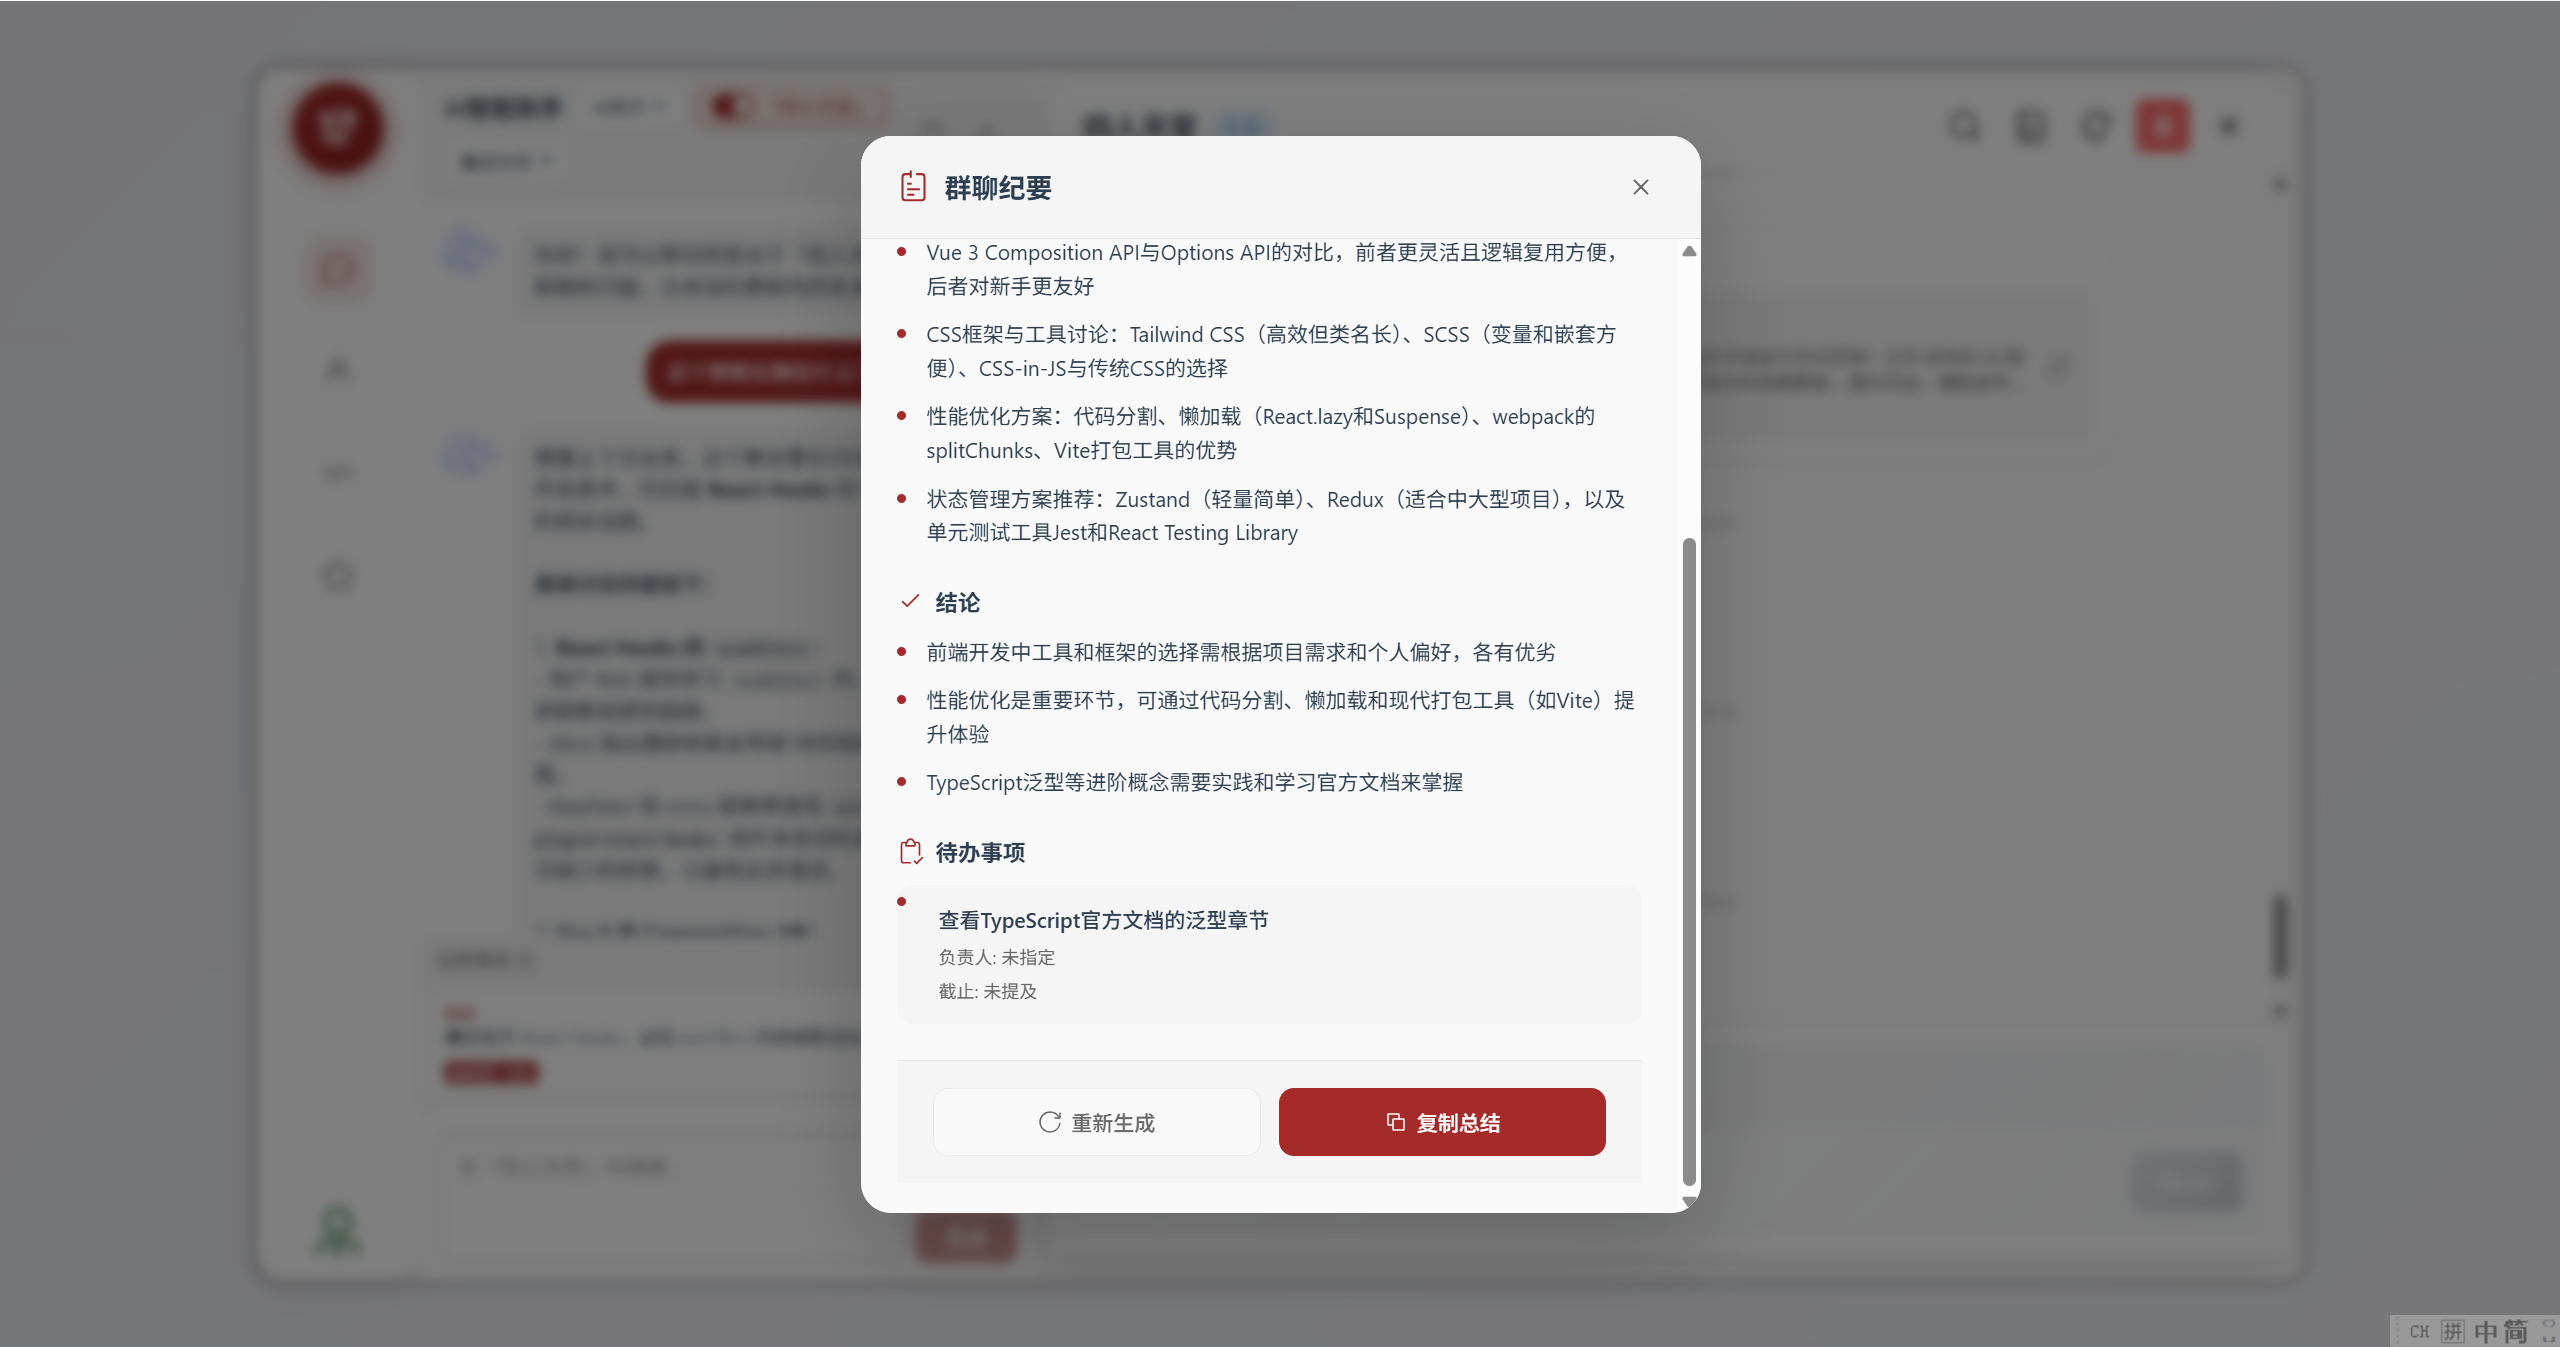
\includegraphics[width=\linewidth,height=4.8cm,keepaspectratio]{img/图6-2_讨论总结结果.png}
\caption{讨论总结结果}
\end{subfigure}
\hfill
\begin{subfigure}[t]{0.48\textwidth}
\centering
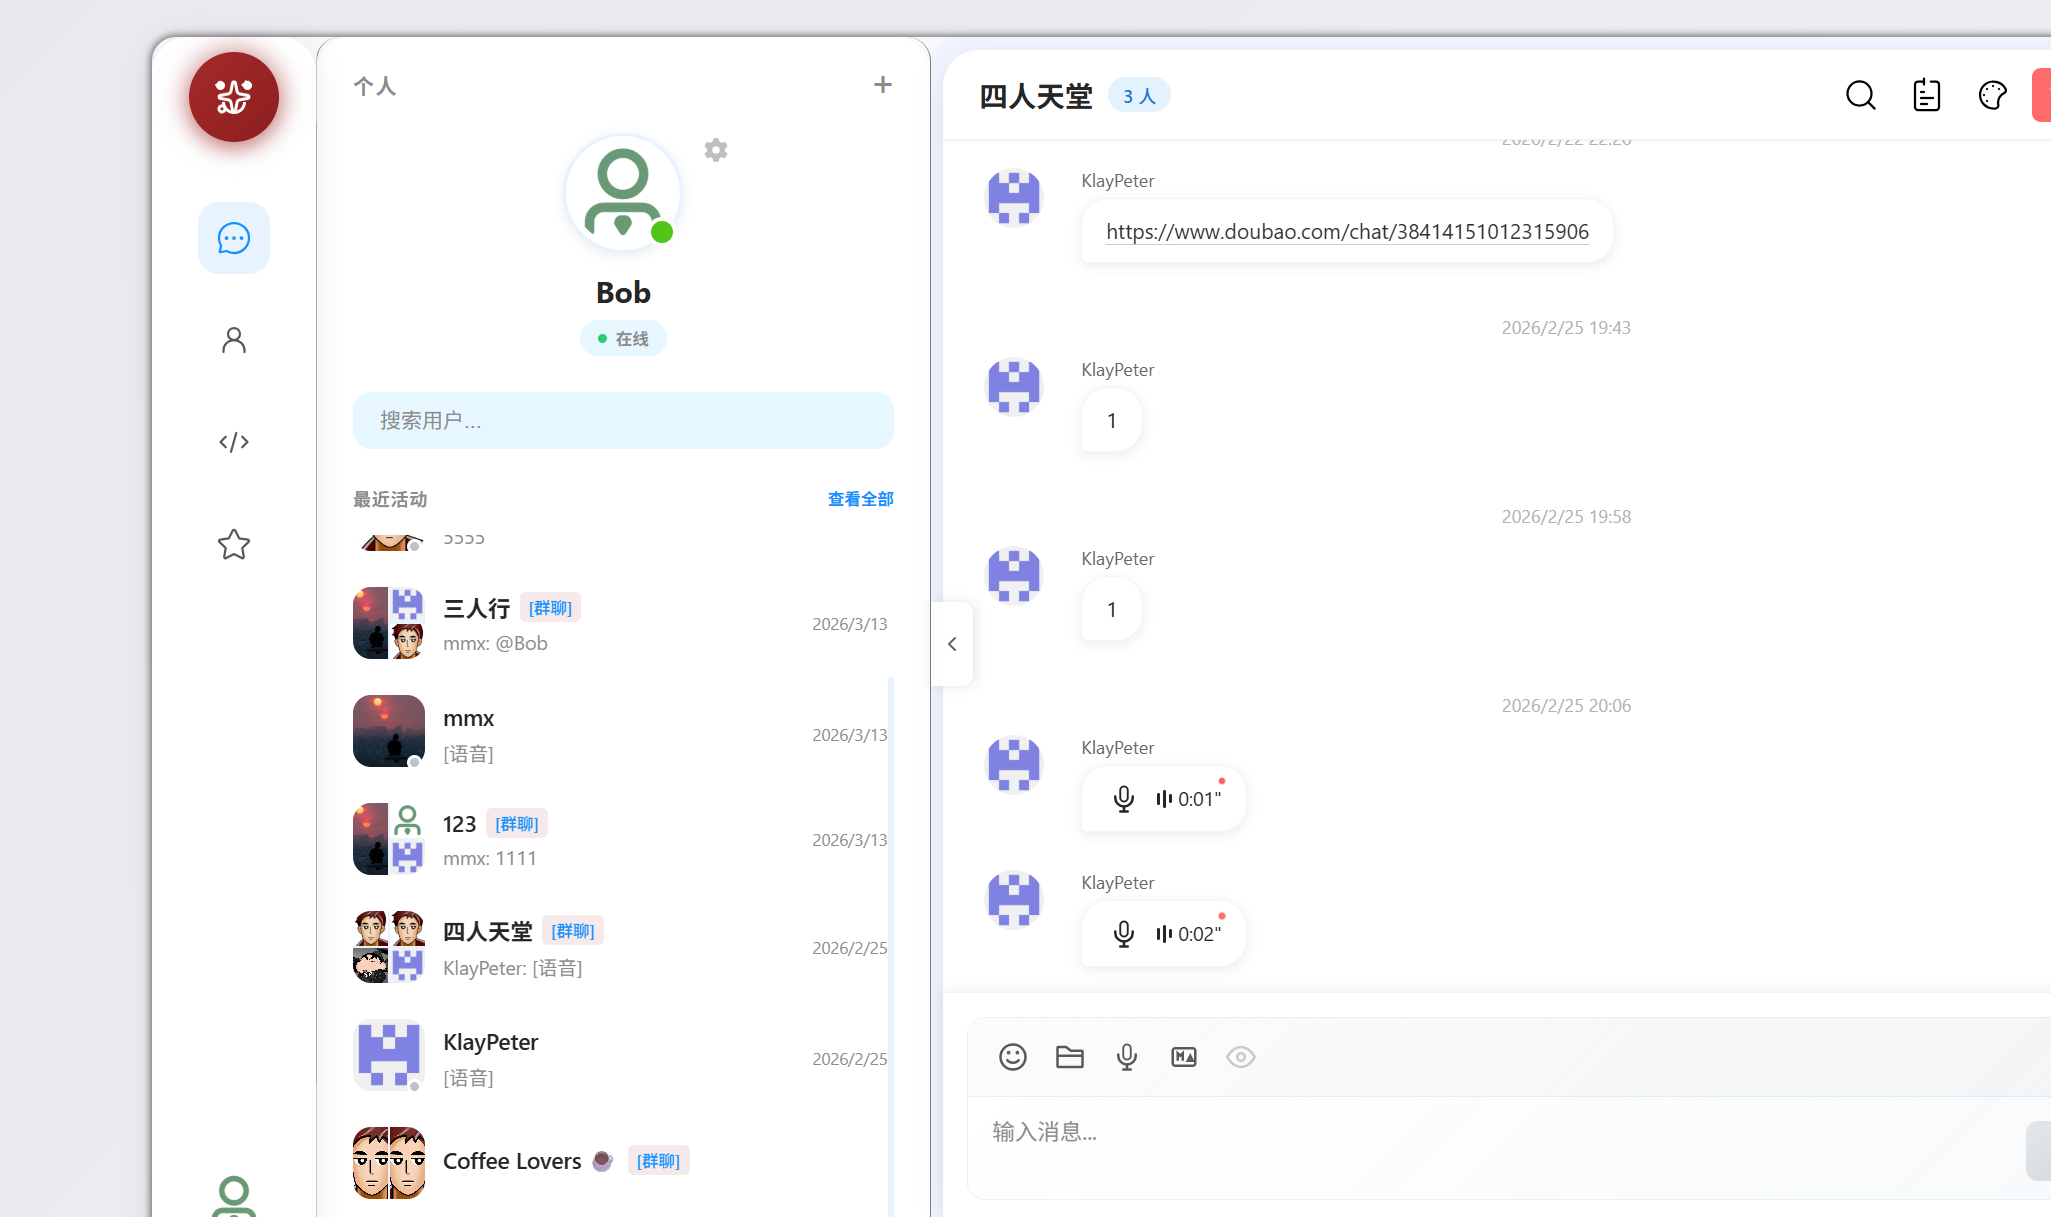
\includegraphics[width=\linewidth,height=4.8cm,keepaspectratio]{img/图6-2_设置与主题切换回显.png}
\caption{设置与主题切换回显}
\end{subfigure}
\caption{Web端功能测试证据组合图}
\label{fig:6-2}
\end{figure}
\FloatBarrier

Web 端功能测试说明，登录、聊天、聊天室、AI 和收藏的主链路已经跑通，但收藏复杂筛选仍然是不稳定点。

\subsection{桌面端功能测试}

桌面端测试以 Windows 打包程序为对象，重点不是重新验证一遍所有功能，而是确认 Web 主链路迁移到 Electron 后仍可用，同时检查托盘、角标、预览和点击跳转这些桌面端特有能力，见表~\ref{tab:6-7}。

\renewcommand{\arraystretch}{1.08}
\setlength{\tabcolsep}{0.55ex}
\small
\begin{longtable}{M{0.12\textwidth}p{0.16\textwidth}p{0.18\textwidth}p{0.18\textwidth}p{0.23\textwidth}}
\testcaselongtablehead{桌面端功能测试用例}{tab:6-7}
DESK-01 & 桌面端启动与登录 & 启动 \texttt{Mini Chat Bar.exe} 并完成登录 & 主窗口正常加载，登录后进入聊天主界面 & 程序可正常启动，登录流程与 Web 端一致 \\
DESK-02 & 托盘驻留 & 点击关闭按钮观察程序行为 & 窗口隐藏到托盘而不是直接退出程序 & 主窗口按设计隐藏，托盘图标仍可保留程序入口 \\
DESK-03 & 未读角标与托盘提示更新 & 触发新消息事件并观察任务栏角标与托盘提示变化 & 未读数更新，窗口获得焦点后清空角标 & 任务栏角标和托盘提示均随未读数变化 \\
DESK-04 & 托盘悬停预览 & 鼠标悬停托盘图标并观察预览窗口 & 弹出预览窗口，显示最近未读会话摘要 & 悬停约 300ms 后弹出预览窗，最多展示最近 5 条未读会话 \\
DESK-05 & 预览点击跳转 & 点击预览窗口中的某条未读消息 & 主窗口恢复并定位到目标会话 & 点击预览项后主窗口被唤起，并定位到对应会话 \\
DESK-06 & 焦点恢复与角标清零 & 点击主窗口或让应用重新获得焦点 & 角标被清空，未读状态与界面同步 & 主窗口恢复焦点后角标被清空，未读状态与界面保持一致 \\
\end{longtable}
\normalsize
\FloatBarrier

桌面端部分重点记录了启动、托盘驻留、未读角标变化、悬停预览和点击跳转五个节点。图~\ref{fig:6-3} 聚焦托盘悬停预览与未读提醒效果，能够直接说明 Electron 侧消息提醒联动正常。

\begin{figure}[H]
\centering
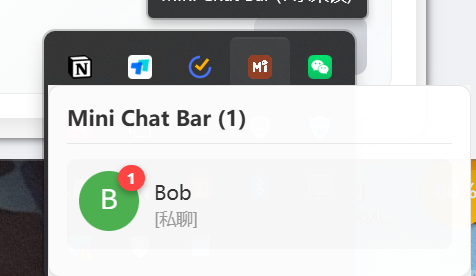
\includegraphics[width=0.46\textwidth]{img/图6-3_桌面端托盘测试.png}
\caption{桌面端功能测试证据图}
\label{fig:6-3}
\end{figure}
\FloatBarrier

结果表明，桌面端已经具备可用的跨端行为：Web 端现有消息链路可以直接复用，托盘提醒和预览跳转也能正常联动。

\subsection{功能测试结果总结}

综合功能测试结果可以认为，当前版本已经跑通了登录、消息、聊天室、AI 和桌面提醒等主要演示链路。当前最明显的问题仍然是收藏组合筛选异常，以及 AI 回答质量受历史语料数量影响。

\section{性能测试}

\subsection{响应时间测试}

性能测试分为响应时间、并发广播和资源占用三部分。响应时间测试先检查日常接口的返回速度，再记录 AI 问答和聊天室总结这类耗时明显更长的调用，量化结果见表~\ref{tab:6-8} 和表~\ref{tab:6-9}。

\renewcommand{\arraystretch}{1.08}
\setlength{\tabcolsep}{0.55ex}
\small
\begin{longtable}{M{0.12\textwidth}p{0.16\textwidth}p{0.18\textwidth}p{0.18\textwidth}p{0.23\textwidth}}
\testcaselongtablehead{响应时间测试用例}{tab:6-8}
PERF-01 & 登录接口响应 & 连续调用登录接口 10 次并记录耗时 & 平均响应时间稳定且无异常失败 & 10 次调用全部成功，平均耗时约 58ms \\
PERF-02 & 用户信息接口响应 & 连续访问用户信息接口 10 次并记录耗时 & 查询接口保持毫秒级返回 & 10 次调用全部成功，平均耗时约 5ms \\
PERF-03 & 聊天室列表接口响应 & 连续访问聊天室列表接口 10 次并记录耗时 & 列表查询稳定返回 & 10 次调用全部成功，平均耗时约 5ms \\
PERF-04 & 消息列表接口响应 & 连续访问消息列表接口 10 次并记录耗时 & 消息读取保持毫秒级返回 & 10 次调用全部成功，平均耗时约 6ms \\
PERF-05 & 收藏列表接口响应 & 连续访问收藏列表接口 10 次并记录耗时 & 收藏页查询稳定返回，不出现超时 & 10 次调用全部成功，平均耗时约 7ms \\
PERF-06 & AI 问答响应 & 调用 AI 问答接口并记录返回时间 & 返回完整回答，不出现超时中断 & 单次耗时约 19.5s，返回约 1500 字内容 \\
PERF-07 & 聊天总结响应 & 调用聊天室总结接口并记录返回时间 & 返回结构化摘要内容 & 单次耗时约 11.8s，基于 5 条消息生成约 600 字摘要 \\
\end{longtable}
\normalsize

\begin{table}[!htbp]
\centering
\caption{响应时间测试结果}
\label{tab:6-9}
\small
\renewcommand{\arraystretch}{1.15}
\setlength{\tabcolsep}{0.8ex}
\begin{tabular}{M{0.20\textwidth}M{0.13\textwidth}M{0.13\textwidth}M{0.13\textwidth}p{0.29\textwidth}}
\toprule
\textbf{测试项} & \textbf{平均值} & \textbf{最小值} & \textbf{最大值} & \textbf{结果分析} \\
\midrule
登录接口 & 58ms & 57ms & 61ms & 认证、密码比对和 JWT 生成均在可接受范围内完成 \\
用户信息接口 & 5ms & 4ms & 6ms & 读取单用户资料开销较小，适合高频调用 \\
聊天室列表接口 & 5ms & 4ms & 7ms & 列表查询结构简单，返回速度稳定 \\
聊天室消息列表接口 & 6.0ms & 5ms & 8ms & 小规模消息分页读取响应平稳 \\
收藏列表接口 & 7ms & 6ms & 9ms & 收藏数量较少时查询稳定，来源名补全未带来明显额外开销 \\
聊天室消息发送接口 & 15ms & -- & -- & 消息写入数据库并广播后仍保持毫秒级返回 \\
私聊消息发送接口 & 11ms & -- & -- & 私聊接口链路较短，返回速度快 \\
私聊 WebSocket 投递 & 6ms & -- & -- & 本地实时消息转发几乎无可感知延迟 \\
AI 问答接口 & 19.5s & -- & -- & 耗时主要来自外部大模型调用，而非本地业务逻辑 \\
聊天室总结接口 & 11.8s & -- & -- & 总结耗时低于 AI 问答，适合阶段性使用而不适合高频触发 \\
\bottomrule
\end{tabular}
\end{table}

\FloatBarrier
表~\ref{tab:6-9} 显示，登录、资料、列表和消息接口都保持在毫秒级；AI 问答约为 19.5s，聊天室总结约为 11.8s。当前性能瓶颈并不在本地 Node 服务，而在外部模型调用。

\subsection{并发性能测试}

并发性能测试主要观察 Socket.IO 在单机环境下的广播表现。测试脚本通过 \texttt{socket.io-client} 建立本地连接，统计平均时延、P95 和最大时延，结果见表~\ref{tab:6-10} 和表~\ref{tab:6-11}。

\renewcommand{\arraystretch}{1.08}
\setlength{\tabcolsep}{0.55ex}
\small
\begin{longtable}{M{0.12\textwidth}p{0.16\textwidth}p{0.18\textwidth}p{0.18\textwidth}p{0.23\textwidth}}
\testcaselongtablehead{并发性能测试用例}{tab:6-10}
CON-01 & 20 客户端广播 & 建立 20 个 Socket 客户端并广播一条群消息 & 所有客户端均能收到消息，广播延迟较低 & 20 个客户端全部收到消息，成功率 100\% \\
CON-02 & 50 客户端广播 & 建立 50 个 Socket 客户端并广播一条群消息 & 所有客户端均能收到消息，不出现掉线 & 50 个客户端全部收到消息，成功率 100\% \\
CON-03 & 100 客户端广播 & 建立 100 个 Socket 客户端并广播一条群消息 & 广播仍能完成，延迟增长保持可控 & 100 个客户端全部收到消息，成功率 100\% \\
CON-04 & 100 客户端连续广播 & 连续发送 10 轮群消息并统计投递情况 & 多轮广播后仍无掉线和明显积压 & 10 轮广播共 1000 次投递均成功，未观察到异常断连 \\
CON-05 & 客户端断线重连后广播 & 广播新消息并观察重连客户端接收情况 & 重连客户端可恢复收消息，在线客户端总数保持稳定 & 重连客户端可再次收到后续广播，房间在线状态恢复正常 \\
\end{longtable}
\normalsize

\begin{table}[!htbp]
\centering
\caption{并发性能测试结果}
\label{tab:6-11}
\small
\renewcommand{\arraystretch}{1.15}
\setlength{\tabcolsep}{0.5ex}
\begin{tabular}{M{0.14\textwidth}M{0.13\textwidth}M{0.13\textwidth}M{0.13\textwidth}M{0.12\textwidth}p{0.20\textwidth}}
\toprule
\textbf{并发客户端数} & \textbf{平均送达时延} & \textbf{P95时延} & \textbf{最大时延} & \textbf{接收成功率} & \textbf{结果分析} \\
\midrule
20 & 3ms & 3ms & 3ms & 100\% & 小规模广播无明显抖动 \\
50 & 3ms & 3ms & 3ms & 100\% & 广播链路稳定，时延未出现明显恶化 \\
100 & 4ms & 5ms & 5ms & 100\% & 单机环境下仍可稳定广播，时延有所上升但整体可控 \\
\bottomrule
\end{tabular}
\end{table}

\FloatBarrier
如图~\ref{fig:6-4}所示，并发广播测试示意图展示了单机环境下 100 客户端广播的主要观测指标。

\begin{figure}[H]
\centering
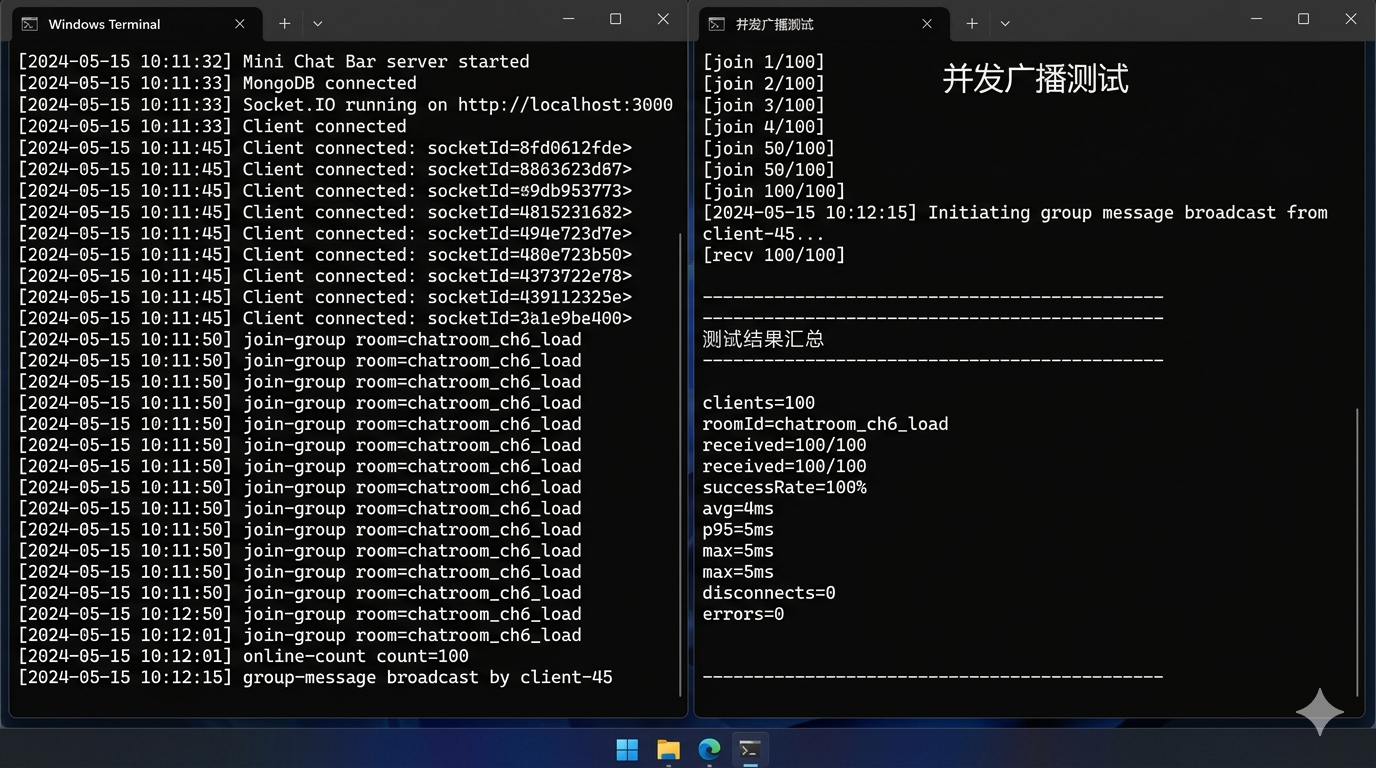
\includegraphics[width=0.92\textwidth]{img/图6-4_并发广播测试日志示意图.png}
\caption{并发广播测试日志示意图}
\label{fig:6-4}
\end{figure}
\FloatBarrier

在 20、50 和 100 个客户端下，广播成功率均为 100\%。单机 100 客户端时平均时延约为 4ms，说明当前规模下广播链路仍然稳定，但这一结果只代表本地环境。

\subsection{资源占用测试}

资源占用测试分别记录 100 客户端广播、单次 AI 问答和单次聊天室总结三种场景下的 CPU 与内存变化，结果见表~\ref{tab:6-12} 和表~\ref{tab:6-13}。

\renewcommand{\arraystretch}{1.08}
\setlength{\tabcolsep}{0.55ex}
\small
\begin{longtable}{M{0.12\textwidth}p{0.16\textwidth}p{0.18\textwidth}p{0.18\textwidth}p{0.23\textwidth}}
\testcaselongtablehead{资源占用测试用例}{tab:6-12}
RES-01 & 广播场景资源占用 & 建立 100 个 Socket 客户端并完成一次群消息广播 & CPU 和内存占用保持在可控范围内，不出现进程异常退出 & 广播测试完成，进程工作集与私有内存均低于 200MB \\
RES-02 & AI 问答场景资源占用 & 对聊天室发起一次完整 AI 问答请求并记录进程占用 & 在等待 AI 返回期间服务进程保持稳定 & AI 请求完成后进程保持正常，内存占用低于 120MB \\
RES-03 & AI 总结场景资源占用 & 对聊天室发起一次完整讨论总结请求并记录进程占用 & 总结生成期间服务进程稳定，无明显资源抖动 & 总结请求完成后进程保持正常，内存占用低于 115MB \\
\end{longtable}
\normalsize

\renewcommand{\arraystretch}{1.15}
\setlength{\tabcolsep}{0.5ex}
\small
\begin{longtable}{M{0.18\textwidth}M{0.12\textwidth}M{0.13\textwidth}M{0.13\textwidth}M{0.13\textwidth}p{0.20\textwidth}}
\resourceusagelongtablehead{资源占用测试结果}{tab:6-13}
100 客户端广播 & 1.5s & 2.1\% & 161MB & 187MB & 连接数增长后内存占用上升，但仍保持在较低水平 \\
单次 AI 问答 & 31.0s & 低于 1\% & 93MB & 118MB & CPU 占用不明显，说明耗时主要消耗在等待外部模型返回 \\
单次 AI 总结 & 12.2s & 低于 1\% & 90MB & 114MB & 与 AI 问答相比总体占用接近，但等待时间更短 \\
\end{longtable}
\normalsize

\FloatBarrier
如图~\ref{fig:6-5}所示，资源占用监测示意图展示了广播压力和 AI 请求压力下的服务端状态差异。

\begin{figure}[H]
\centering
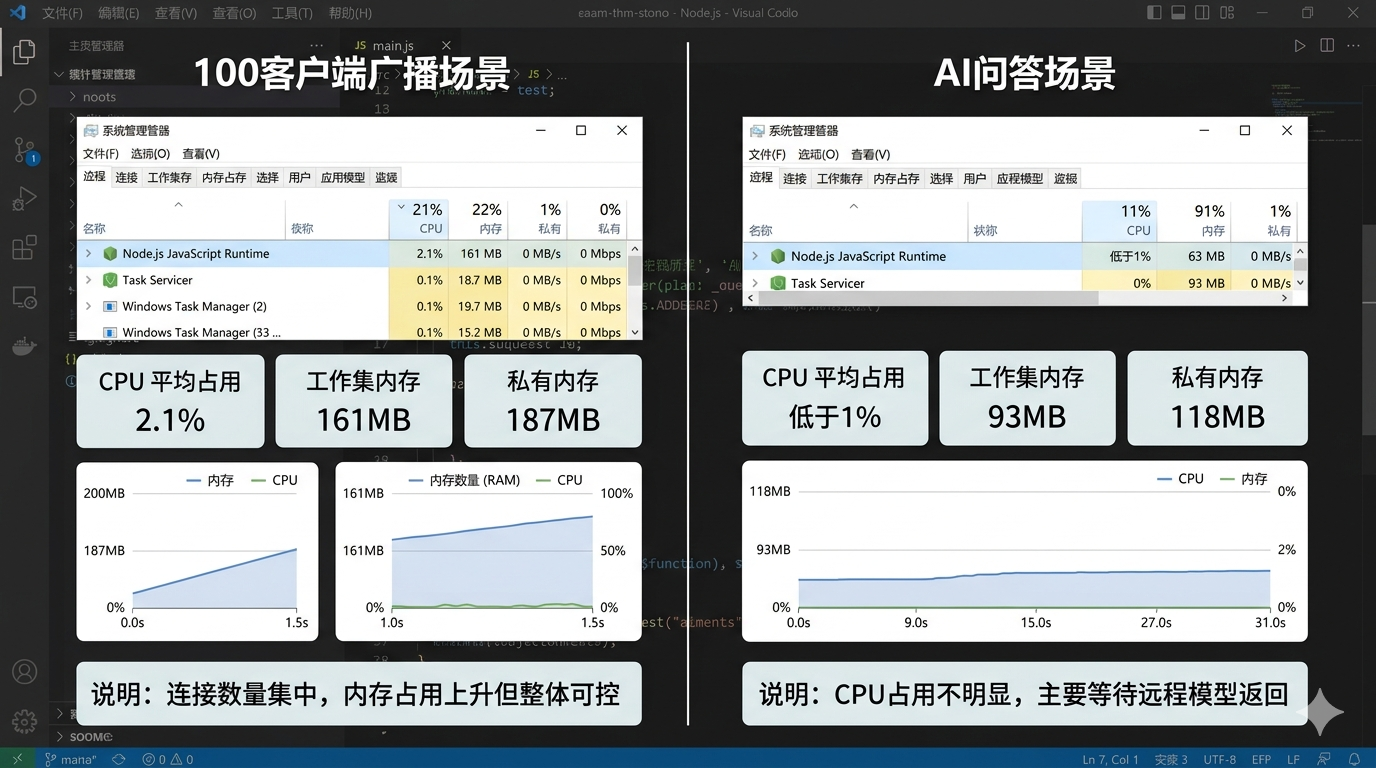
\includegraphics[width=0.92\textwidth]{img/图6-5_资源占用监测示意图.png}
\caption{资源占用监测示意图}
\label{fig:6-5}
\end{figure}
\FloatBarrier

资源监测结果说明，广播场景主要抬高内存占用，AI 场景则更多消耗等待时间。本地服务端 CPU 压力不高，说明 AI 耗时主要来自等待外部模型返回。

\subsection{性能测试结果总结}

综合响应时间、并发广播和资源占用结果，系统在当前单机部署下已经能满足课程项目和答辩演示。普通接口、消息列表读取和 Socket 广播都保持了较稳定的响应水平，说明当前前后端主链路在小规模本地环境下可以支撑连续展示与演示操作。

从性能瓶颈分布看，当前最主要的耗时来源仍然是外部模型调用，而不是本地 Node 服务与数据库访问；从资源曲线看，广播场景主要推高内存占用，AI 场景则更多体现在等待时间拉长。后续需要优先处理的仍是 AI 耗时和收藏复杂筛选这两个边界问题，同时也应继续关注更高并发和更长时段运行下的稳定性变化。
